\documentclass[aspectratio=169]{beamer}

\usetheme{Madrid}
\usecolortheme{default}
\setbeamertemplate{navigation symbols}{}

\usepackage[T5,T1]{fontenc}
\usepackage[utf8]{inputenc}
\usepackage[english,vietnamese]{babel}
\usepackage{graphicx}
\usepackage{booktabs}
\usepackage{tikz}
\usepackage{amsmath,amssymb}
\usepackage{subcaption}

\definecolor{accent}{RGB}{14,88,109}
\definecolor{soft}{RGB}{236,244,247}
\setbeamercolor{title}{fg=white,bg=accent}
\setbeamercolor{subtitle}{fg=accent}
\setbeamercolor{frametitle}{fg=white,bg=accent}
\setbeamercolor{structure}{fg=accent}
\setbeamercolor{block title}{fg=white,bg=accent}
\setbeamercolor{block body}{bg=soft}

\graphicspath{{figures/}}

\title[Sparse-View RGB + Estimated Depth]{Sparse-View RGB 3D Scene Reconstruction\\with Fine-Tuned Estimated-Depth Correction}
\author[CV Team]{Nguyễn Ngọc Minh, Kiều Sơn Tùng, Đặng Thịnh Tường Minh}
\institute[IT4343E]{IT4343E - Computer Vision}
\date{June 2026}

\begin{document}

\begin{frame}
    \titlepage
\end{frame}

\begin{frame}{Table of Contents}
    \tableofcontents
\end{frame}

\section{Introduction}

\begin{frame}{What is 3D Reconstruction?}
    \begin{itemize}
        \item \textbf{Definition:} The process of capturing the shape and appearance of real-world objects or environments to create digital 3D models.
        \item \textbf{Applications:} Augmented reality, robotics navigation, digital twins, and indoor mapping.
        \item \textbf{Practical Challenge:} Classical pipelines require dense, overlapping images, calibrated cameras, and known depth. 
        \item \textbf{Our Goal:} Reconstruct high-quality 3D indoor scenes from a strictly \textbf{sparse set} (3-5 views) of ordinary 2D RGB images, mimicking a user snapping a few photos with a phone.
    \end{itemize}
\end{frame}

\section{Background and Limitations}

\begin{frame}{MV-DUSt3R+ and its Limitations}
    \begin{columns}
        \begin{column}{0.5\textwidth}
            \textbf{What is MV-DUSt3R+?}
            \begin{itemize}
                \item A state-of-the-art feed-forward model that reconstructs scenes directly from sparse RGB views.
                \item Uses cross-view reasoning to output candidate 3D geometry without external camera poses.
            \end{itemize}
            \vspace{0.2cm}
            \centering
            
\includegraphics[width=0.8\linewidth]{mv_overview.png}
        \end{column}
        \begin{column}{0.5\textwidth}
            \begin{block}{Limitations of Pure RGB}
                \begin{itemize}
                    \item \textbf{Scale Ambiguity:} The output is in an arbitrary coordinate space. It cannot determine if a room is 2 meters or 20 meters wide.
                    \item \textbf{Geometric Instability:} Fails on textureless walls and reflective surfaces, causing flat surfaces to "fold" and producing floating points in mid-air.
                \end{itemize}
            \end{block}
        \end{column}
    \end{columns}
\end{frame}

\section{Proposed Method}

\begin{frame}{Solving it with a Depth Model}
    To fix MV-DUSt3R+, we extract its rigid camera poses and combine them with a \textbf{Fine-Tuned Depth Model} (DepthAnything V2) which acts as a physical mold.
    \vspace{0.2cm}
    \begin{columns}
        \begin{column}{0.5\textwidth}
            \textbf{1. Depth Anchor Projection:}
            \begin{equation*}
                X_{\mathrm{depth}}^{\mathrm{world}} = T_i \left( \hat{D}_i K_i^{-1}\begin{bmatrix}u\\v\\1\end{bmatrix} \right)
            \end{equation*}
            \small (We project the metric depth map $\hat{D}_i$ into 3D using the MV-DUSt3R+ pose $T_i$)
        \end{column}
        \begin{column}{0.5\textwidth}
            \textbf{2. Geometric Correction:}
            \begin{equation*}
                r = \| X_{\mathrm{mv}} - X_{\mathrm{depth}}^{\mathrm{world}} \|_2
            \end{equation*}
            \begin{equation*}
                X_{\mathrm{corr}} = (1-\alpha)X_{\mathrm{mv}} + \alpha X_{\mathrm{depth}}^{\mathrm{world}}
            \end{equation*}
            \small (If the residual $r \geq \tau$, we blend the folded candidate point into the structured metric anchor.)
        \end{column}
    \end{columns}
\end{frame}

\section{Dataset}

\begin{frame}{Dataset: ScanNet Overview}
    \begin{columns}
        \begin{column}{0.5\textwidth}
            \begin{itemize}
                \item \textbf{Source Dataset:} Derived from ScanNet (captured with iPad Air 2).
                \item \textbf{Environment:} Typical indoor scenes (offices, bedrooms) with heavy furniture occlusion and reflective surfaces.
                \item \textbf{Contents:} Provides aligned RGB and active depth frames, optimized poses, and dense 3D meshes.
                \item \textbf{Our Sparse Input:} We artificially restrict the system to use only 3 to 5 RGB images at inference time.
            \end{itemize}
        \end{column}
        \begin{column}{0.5\textwidth}
            \centering
            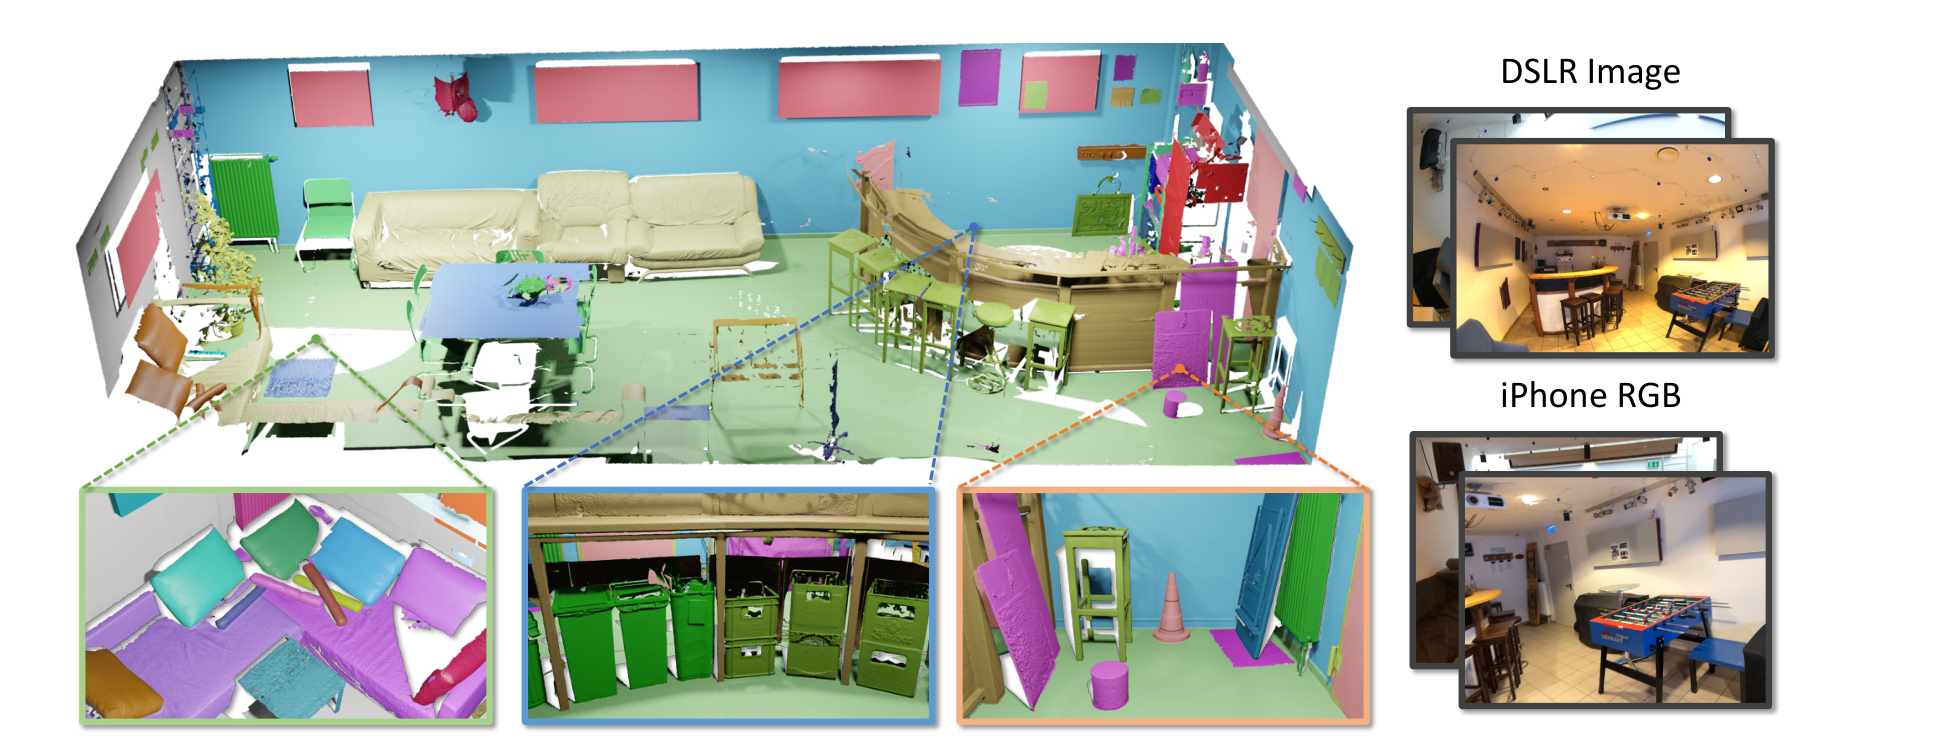
\includegraphics[width=\textwidth]{scannetpp_overview_crop.png}
        \end{column}
    \end{columns}
\end{frame}

\section{Experimental Setting}

\begin{frame}{Experimental Setting}
    \begin{itemize}
        \item \textbf{Deployment Constraint:} The entire inference pipeline operates purely on sparse RGB images. The measured ScanNet depth is \textbf{only} used to fine-tune the depth estimator and for final ground truth evaluation.
        \item \textbf{Hardware:} All inference and fine-tuning processes are executed in a controlled Kaggle notebook environment equipped with NVIDIA GPUs.
        \item \textbf{Inputs:}
    \end{itemize}
    \vspace{0.2cm}
    \begin{figure}
        \centering
        \begin{subfigure}[b]{0.24\textwidth}
            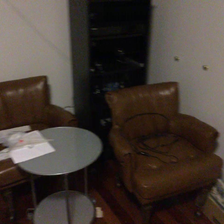
\includegraphics[width=\textwidth]{dataset_1.png}
        \end{subfigure}
        \hfill
        \begin{subfigure}[b]{0.24\textwidth}
            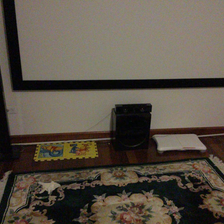
\includegraphics[width=\textwidth]{dataset_2.png}
        \end{subfigure}
        \hfill
        \begin{subfigure}[b]{0.24\textwidth}
            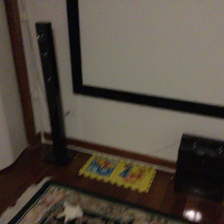
\includegraphics[width=\textwidth]{dataset_3.png}
        \end{subfigure}
        \hfill
        \begin{subfigure}[b]{0.24\textwidth}
            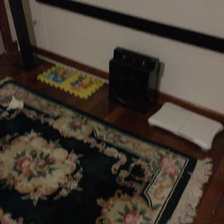
\includegraphics[width=\textwidth]{dataset_4.png}
        \end{subfigure}
        \caption{Sparse 4-view RGB input group fed into the deployment pipeline.}
    \end{figure}
\end{frame}

\section{Evaluation}

\begin{frame}{Evaluation Metrics}
    \begin{columns}
        \begin{column}{0.4\textwidth}
            \begin{figure}
                \centering
                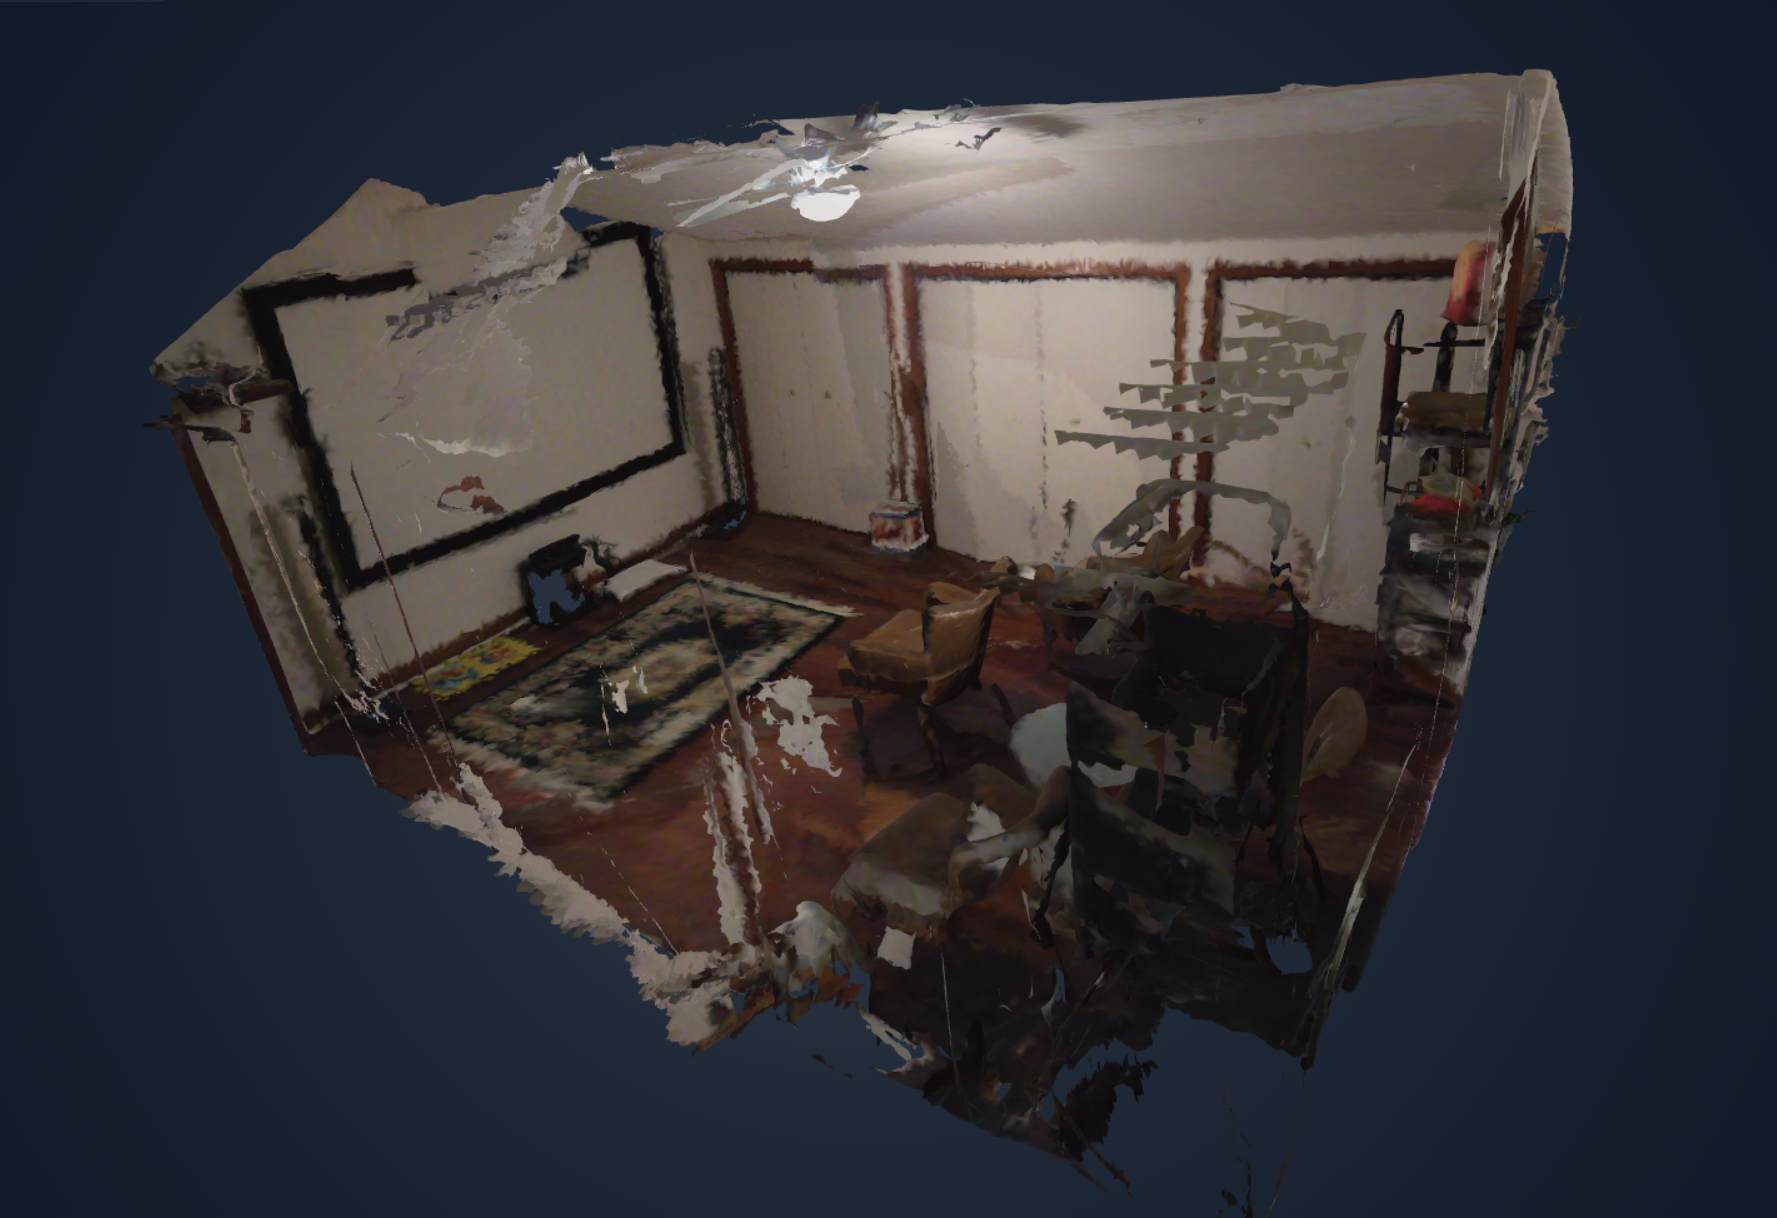
\includegraphics[width=\textwidth]{3D_GT.png}
                \caption{Ground Truth 3D Structure used strictly as an upper-bound reference.}
            \end{figure}
        \end{column}
        \begin{column}{0.6\textwidth}
            \textbf{Depth Estimation Metrics}
            \begin{itemize}
                \item AbsRel, MAE, RMSE, $\delta_1$ accuracy.
            \end{itemize}
            \vspace{0.3cm}
            \textbf{Point-Cloud Reconstruction Metrics}
            \begin{itemize}
                \item \textbf{Accuracy:} Distance from Prediction to GT.
                \item \textbf{Completeness:} Distance from GT to Prediction.
                \item \textbf{Chamfer Distance:} Symmetric geometric deviation.
                \item \textbf{F-score:} Overall geometric fidelity.
            \end{itemize}
        \end{column}
    \end{columns}
\end{frame}

\section{Conclusion}

\begin{frame}{Conclusion}
    \begin{itemize}
        \item \textbf{Deployability:} Successfully reconstructs metric 3D scenes from a few standard RGB photos, avoiding the need for specialized depth sensors.
        \item \textbf{Geometric Stability:} The fine-tuned depth estimator effectively acts as a physical mold to fix "folded" walls and floating artifacts inherent to pure RGB-matching models.
        \item \textbf{Absolute Scale:} Naturally resolves the scale ambiguity of MV-DUSt3R+, producing outputs in real-world physical meters suitable for downstream robotics and AR tasks.
    \end{itemize}
    \vspace{0.5cm}
    \begin{center}
        \Large \textbf{Thank You!}
    \end{center}
\end{frame}

\end{document}
